\documentclass[]{article}
\usepackage{lmodern}
\usepackage{amssymb,amsmath}
\usepackage{ifxetex,ifluatex}
\usepackage{fixltx2e} % provides \textsubscript
\ifnum 0\ifxetex 1\fi\ifluatex 1\fi=0 % if pdftex
  \usepackage[T1]{fontenc}
  \usepackage[utf8]{inputenc}
\else % if luatex or xelatex
  \ifxetex
    \usepackage{mathspec}
  \else
    \usepackage{fontspec}
  \fi
  \defaultfontfeatures{Ligatures=TeX,Scale=MatchLowercase}
\fi
% use upquote if available, for straight quotes in verbatim environments
\IfFileExists{upquote.sty}{\usepackage{upquote}}{}
% use microtype if available
\IfFileExists{microtype.sty}{%
\usepackage{microtype}
\UseMicrotypeSet[protrusion]{basicmath} % disable protrusion for tt fonts
}{}
\usepackage[margin=1in]{geometry}
\usepackage{hyperref}
\hypersetup{unicode=true,
            pdftitle={README for random forest (RF)},
            pdfauthor={Group 2},
            pdfborder={0 0 0},
            breaklinks=true}
\urlstyle{same}  % don't use monospace font for urls
\usepackage{color}
\usepackage{fancyvrb}
\newcommand{\VerbBar}{|}
\newcommand{\VERB}{\Verb[commandchars=\\\{\}]}
\DefineVerbatimEnvironment{Highlighting}{Verbatim}{commandchars=\\\{\}}
% Add ',fontsize=\small' for more characters per line
\usepackage{framed}
\definecolor{shadecolor}{RGB}{248,248,248}
\newenvironment{Shaded}{\begin{snugshade}}{\end{snugshade}}
\newcommand{\AlertTok}[1]{\textcolor[rgb]{0.94,0.16,0.16}{#1}}
\newcommand{\AnnotationTok}[1]{\textcolor[rgb]{0.56,0.35,0.01}{\textbf{\textit{#1}}}}
\newcommand{\AttributeTok}[1]{\textcolor[rgb]{0.77,0.63,0.00}{#1}}
\newcommand{\BaseNTok}[1]{\textcolor[rgb]{0.00,0.00,0.81}{#1}}
\newcommand{\BuiltInTok}[1]{#1}
\newcommand{\CharTok}[1]{\textcolor[rgb]{0.31,0.60,0.02}{#1}}
\newcommand{\CommentTok}[1]{\textcolor[rgb]{0.56,0.35,0.01}{\textit{#1}}}
\newcommand{\CommentVarTok}[1]{\textcolor[rgb]{0.56,0.35,0.01}{\textbf{\textit{#1}}}}
\newcommand{\ConstantTok}[1]{\textcolor[rgb]{0.00,0.00,0.00}{#1}}
\newcommand{\ControlFlowTok}[1]{\textcolor[rgb]{0.13,0.29,0.53}{\textbf{#1}}}
\newcommand{\DataTypeTok}[1]{\textcolor[rgb]{0.13,0.29,0.53}{#1}}
\newcommand{\DecValTok}[1]{\textcolor[rgb]{0.00,0.00,0.81}{#1}}
\newcommand{\DocumentationTok}[1]{\textcolor[rgb]{0.56,0.35,0.01}{\textbf{\textit{#1}}}}
\newcommand{\ErrorTok}[1]{\textcolor[rgb]{0.64,0.00,0.00}{\textbf{#1}}}
\newcommand{\ExtensionTok}[1]{#1}
\newcommand{\FloatTok}[1]{\textcolor[rgb]{0.00,0.00,0.81}{#1}}
\newcommand{\FunctionTok}[1]{\textcolor[rgb]{0.00,0.00,0.00}{#1}}
\newcommand{\ImportTok}[1]{#1}
\newcommand{\InformationTok}[1]{\textcolor[rgb]{0.56,0.35,0.01}{\textbf{\textit{#1}}}}
\newcommand{\KeywordTok}[1]{\textcolor[rgb]{0.13,0.29,0.53}{\textbf{#1}}}
\newcommand{\NormalTok}[1]{#1}
\newcommand{\OperatorTok}[1]{\textcolor[rgb]{0.81,0.36,0.00}{\textbf{#1}}}
\newcommand{\OtherTok}[1]{\textcolor[rgb]{0.56,0.35,0.01}{#1}}
\newcommand{\PreprocessorTok}[1]{\textcolor[rgb]{0.56,0.35,0.01}{\textit{#1}}}
\newcommand{\RegionMarkerTok}[1]{#1}
\newcommand{\SpecialCharTok}[1]{\textcolor[rgb]{0.00,0.00,0.00}{#1}}
\newcommand{\SpecialStringTok}[1]{\textcolor[rgb]{0.31,0.60,0.02}{#1}}
\newcommand{\StringTok}[1]{\textcolor[rgb]{0.31,0.60,0.02}{#1}}
\newcommand{\VariableTok}[1]{\textcolor[rgb]{0.00,0.00,0.00}{#1}}
\newcommand{\VerbatimStringTok}[1]{\textcolor[rgb]{0.31,0.60,0.02}{#1}}
\newcommand{\WarningTok}[1]{\textcolor[rgb]{0.56,0.35,0.01}{\textbf{\textit{#1}}}}
\usepackage{longtable,booktabs}
\usepackage{graphicx,grffile}
\makeatletter
\def\maxwidth{\ifdim\Gin@nat@width>\linewidth\linewidth\else\Gin@nat@width\fi}
\def\maxheight{\ifdim\Gin@nat@height>\textheight\textheight\else\Gin@nat@height\fi}
\makeatother
% Scale images if necessary, so that they will not overflow the page
% margins by default, and it is still possible to overwrite the defaults
% using explicit options in \includegraphics[width, height, ...]{}
\setkeys{Gin}{width=\maxwidth,height=\maxheight,keepaspectratio}
\IfFileExists{parskip.sty}{%
\usepackage{parskip}
}{% else
\setlength{\parindent}{0pt}
\setlength{\parskip}{6pt plus 2pt minus 1pt}
}
\setlength{\emergencystretch}{3em}  % prevent overfull lines
\providecommand{\tightlist}{%
  \setlength{\itemsep}{0pt}\setlength{\parskip}{0pt}}
\setcounter{secnumdepth}{0}
% Redefines (sub)paragraphs to behave more like sections
\ifx\paragraph\undefined\else
\let\oldparagraph\paragraph
\renewcommand{\paragraph}[1]{\oldparagraph{#1}\mbox{}}
\fi
\ifx\subparagraph\undefined\else
\let\oldsubparagraph\subparagraph
\renewcommand{\subparagraph}[1]{\oldsubparagraph{#1}\mbox{}}
\fi

%%% Use protect on footnotes to avoid problems with footnotes in titles
\let\rmarkdownfootnote\footnote%
\def\footnote{\protect\rmarkdownfootnote}

%%% Change title format to be more compact
\usepackage{titling}

% Create subtitle command for use in maketitle
\providecommand{\subtitle}[1]{
  \posttitle{
    \begin{center}\large#1\end{center}
    }
}

\setlength{\droptitle}{-2em}

  \title{README for random forest (RF)}
    \pretitle{\vspace{\droptitle}\centering\huge}
  \posttitle{\par}
    \author{Group 2}
    \preauthor{\centering\large\emph}
  \postauthor{\par}
      \predate{\centering\large\emph}
  \postdate{\par}
    \date{02 12 2019}


\begin{document}
\maketitle

\textbf{Corresponding R Script:}
\href{https://github.com/NicSchuler/DSF_NFLDraftPrediction/blob/master/Project_Scripts/RandomForest.R}{RF}

\hypertarget{introduction}{%
\section{1. Introduction}\label{introduction}}

The goal of this project is to make a prediction about the likelilhood
of College Football (CFB) players to be drafted into the professional
football league (NFL). In order to achieve this, different aspects of a
CFB player's college career are being used as features
\(p_{1}, ..., p_{n}\). These include game statistics such as rush
attempts \texttt{Rush.Att} or yards ran after a pass \texttt{Pass.Yard}.
To solve this problem, one of the methods employed is a random forest
classifier (RF). RF is an ensemble learning method (a method comprised
of different methods) that constructs multiple small decision trees that
are ineffective on their own but exceedingly effective when combining
the individual trees to output the class which is the mode of all
individually predicted classes. Through this process of combining
individually ``useless'' trees into a ``forest'', this model is very
effective in combatting overfitting the training set (i.e.~learning very
specific patterns in the training data and therefore showing low bias
but high variance) which is prevalent in regular decision tree models.

\hypertarget{bootstrap-aggregation-and-feature-bagging}{%
\section{2. Bootstrap aggregation and feature
bagging}\label{bootstrap-aggregation-and-feature-bagging}}

In order to build the individual decision trees within the RF model,
bootstrap aggregation (bagging) is conducted. This process assembles
individual sample bags \(X_{b}\) and labels \(Y_{b}\) of training data
through drawing randomly with replacement from the entire pool of
training data \(x_{1},...,x_{n}\) with the corresponding labels
\(y_{1},...,y_{n}\). For every one of these bags \(b=1,...,B\), a
classification (or regression) decision tree \(f_{b}\) is fitted and
subsequently the majority vote is used in classification problems or
averaged over all bags \(b\) in regression problems:

\[\hat{f}=\frac{1}{B}\sum_{b=1}^{B} f_{b}(X_{b})\] This process of using
many smaller and ``less intelligent'' trees in combination reduces
variance by prohibiting one single tree of fitting the entire training
set too closely. This would come at the cost of a higher bias when
simply training many smaller trees on correlated samples of training
data. Because the bags are assembled randomly with replacement,
bootstrapping de-correlates the individual bags which in turn allows the
RF model to reduce variance without increasing bias.

The second measure to enhance RF performance used on top of
bootstrapping is sample bagging. Through the random selection of a
subset of features to train on for every tree in the model, correlation
between the trees is further reduced. If certain features are very
strong predictors of the ouput, using them on all sub-trees would
correlate them and therefore yield a higher bias. In the script, the
default value of features for classification \(\sqrt{p}\) is passed as
the \texttt{mtry} argument due to time constraints of this project and
the increase of computing time associated with extended tuning, however
the optimal number depends on the training data and should therefore be
treated as a tuning parameter in the future.

\hypertarget{data-standardization}{%
\section{3. Data Standardization}\label{data-standardization}}

Because the goal of RF is to obtain a set of partition rules to make a
classification decision, it is not sensitive to differently scaled or
centered features and therefore does not change depending on monotonic
transformation of the input data. This means that there is no need to
standardize the data used, event though it is differently scaled across
features (see
\href{https://github.com/NicSchuler/DSF_NFLDraftPrediction/tree/master/Data/READMEs}{RM\_DataHandling})

\hypertarget{tuning-the-model}{%
\section{4. Tuning the model}\label{tuning-the-model}}

In this project 10-fold cross validation was used to determine the
optimal number of trees (\texttt{ntree}) to use in the RF model. For
every position (\texttt{QB}, \texttt{RB}, \texttt{WR} and \texttt{all}),
10 folds of training data were fitted to an iteration of the RF model
and its performance was tested. In the R script this is realized in the
\texttt{perfFun(x)} function:

\begin{Shaded}
\begin{Highlighting}[]
\NormalTok{perfFun <-}\StringTok{ }\ControlFlowTok{function}\NormalTok{(TP, FP, TN, FN)\{}
\NormalTok{  accuracy <-}\StringTok{ }\NormalTok{(TP }\OperatorTok{+}\StringTok{ }\NormalTok{TN)}\OperatorTok{/}\NormalTok{(TP }\OperatorTok{+}\StringTok{ }\NormalTok{FP }\OperatorTok{+}\StringTok{ }\NormalTok{TN }\OperatorTok{+}\StringTok{ }\NormalTok{FN)}
\NormalTok{  precision <-}\StringTok{ }\NormalTok{TP}\OperatorTok{/}\NormalTok{(TP }\OperatorTok{+}\StringTok{ }\NormalTok{FP)}
\NormalTok{  recall <-}\StringTok{ }\NormalTok{TP}\OperatorTok{/}\NormalTok{(TP }\OperatorTok{+}\StringTok{ }\NormalTok{FN)}
\NormalTok{  F1 <-}\StringTok{ }\DecValTok{2}\OperatorTok{*}\NormalTok{((precision}\OperatorTok{*}\NormalTok{recall)}\OperatorTok{/}\NormalTok{(precision }\OperatorTok{+}\StringTok{ }\NormalTok{recall))}
\NormalTok{  out <-}\StringTok{ }\KeywordTok{data.frame}\NormalTok{(}\StringTok{"Accuracy"}\NormalTok{ =}\StringTok{ }\NormalTok{accuracy, }\StringTok{"Precision"}\NormalTok{ =}\StringTok{ }\NormalTok{precision, }\StringTok{"Recall"}\NormalTok{ =}\StringTok{ }\NormalTok{recall, }\StringTok{"F1"}\NormalTok{ =}\StringTok{ }\NormalTok{F1)}
  \KeywordTok{return}\NormalTok{(out)}
\NormalTok{\}}
\end{Highlighting}
\end{Shaded}

To limit computation time, only 10 intervals of 100 trees were tested,
which leaves the possibility of better performance when testing on a
more granular level. As discussed above, an additional parameter to tune
would be the number of features used in the feature bagging process.

\hypertarget{implementation-in-r}{%
\section{5. Implementation in R}\label{implementation-in-r}}

The application of RF in R is explained below. All code is included in
the
\href{https://github.com/NicSchuler/DSF_NFLDraftPrediction/blob/master/Project_Scripts/RandomForest.R}{RF
script} and step-by-step comments are provided.

\hypertarget{training-the-rf-model}{%
\subsection{5.1 Training the RF Model}\label{training-the-rf-model}}

For training the data from years 2007 to 2013 of all unsampled and
sampled datasets are used respectively. The RF model is built and
trained using the \texttt{randomForest} package. As previouly described,
the model is tuned for the optimal number of trees to use, which is
passed as the \texttt{ntrees} parameter to the \texttt{ntree\ =}
argument.

\begin{Shaded}
\begin{Highlighting}[]
\NormalTok{RF_QB <-}\StringTok{ }\KeywordTok{randomForest}\NormalTok{(y }\OperatorTok{~}\StringTok{ }\NormalTok{., }\DataTypeTok{data =}\NormalTok{ x, }\DataTypeTok{ntree =}\NormalTok{ ntrees)}
\end{Highlighting}
\end{Shaded}

To make predictions for the testing data, the
\texttt{predict.randomForest} function is used. For the probability
cutoff value 0.5 is used by default. Because the project works with
classification, this value is the fraction of votes for one of the
classes, so a cutoff of 0.5 can be understood as a majority vote by the
different features.

\begin{Shaded}
\begin{Highlighting}[]
\NormalTok{pred <-}\StringTok{ }\KeywordTok{as.integer}\NormalTok{(}\KeywordTok{as.vector}\NormalTok{(}\KeywordTok{predict}\NormalTok{(RF_QB, x_test)))}
\end{Highlighting}
\end{Shaded}

\hypertarget{variable-importance}{%
\subsection{5.2 Variable Importance}\label{variable-importance}}

The RF model can be used to determine variable importance. To achieve
this, a RF is fitted to the data, features are subsequently perturbated
individually and the change in average out-of-bag (OOB) error is
compared among the features. The resulting comparison allows for
statements about the variable importance (i.e.~the feature yielding the
biggest difference in OOB error having the greatest impact). To
visualize variable importance in this project, the Mean Decrease in Gini
for all features was plotted for all positions and all sampling methods.
Higher Mean Decrease in Gini indicates higher variable importance.

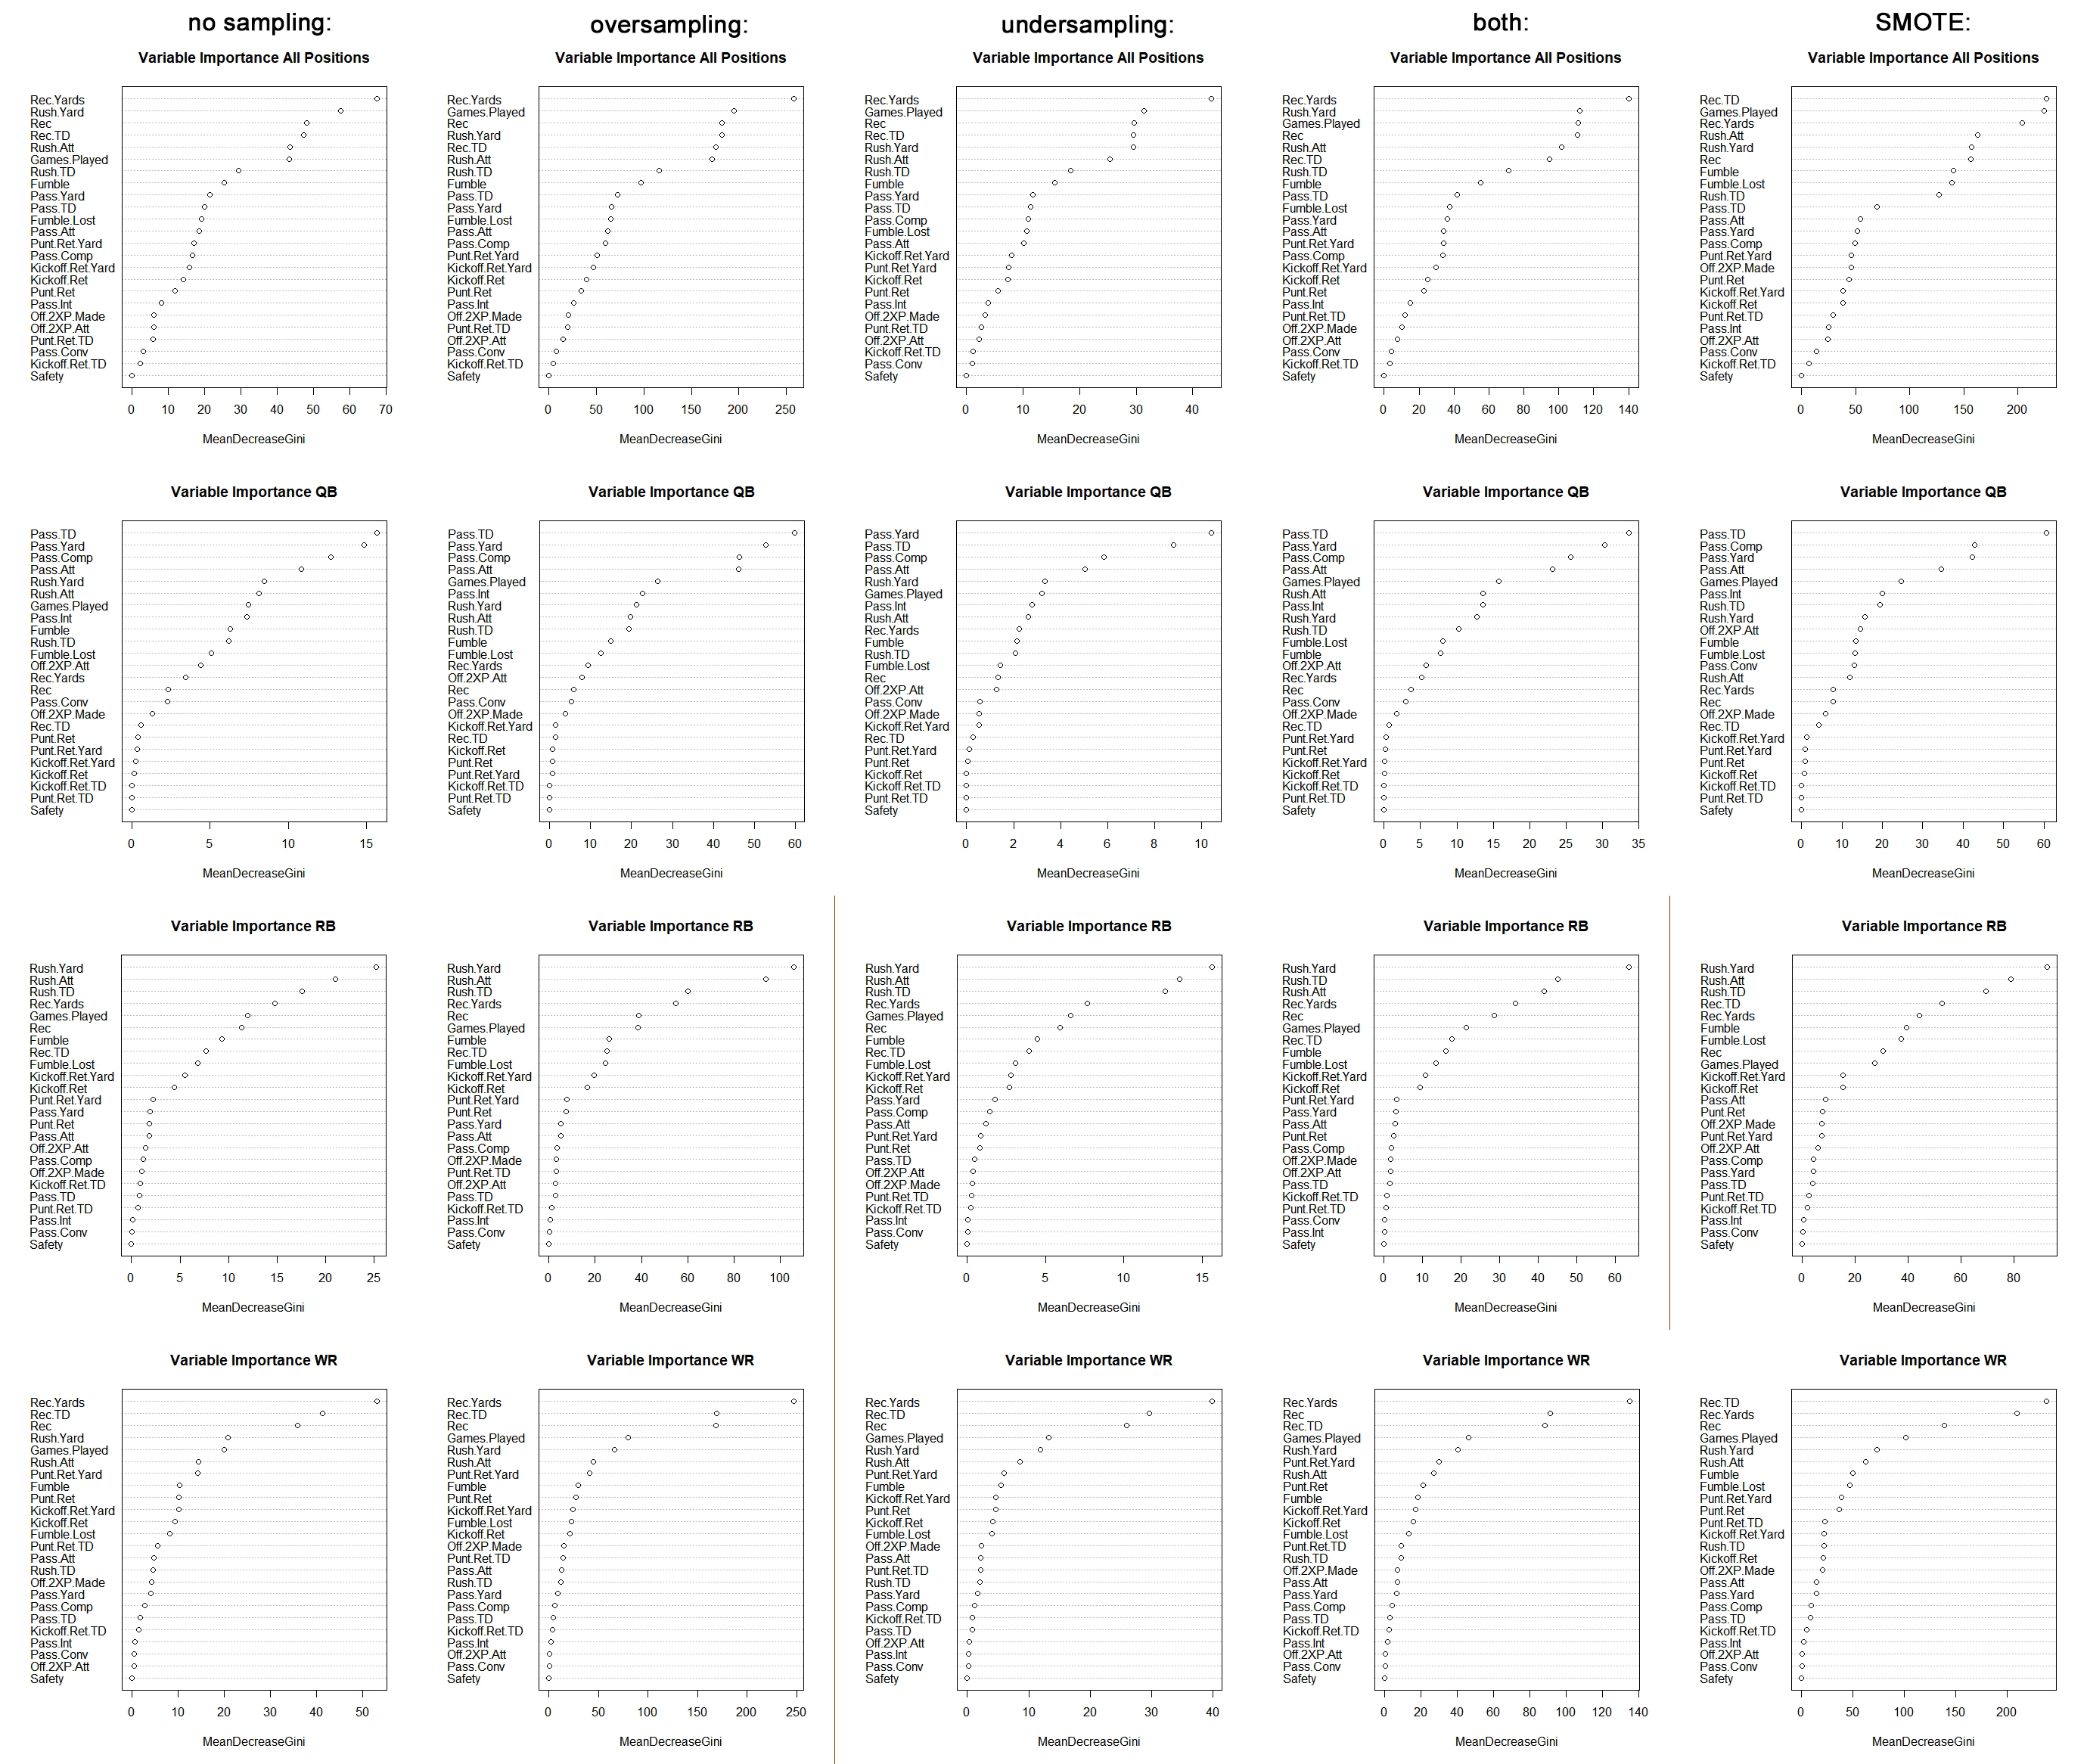
\includegraphics{RM_randomForest_files/variable_importance.jpg}

Because the datasets do not include categorical variables with multiple
levels, variable importance is not biased towards features with more
levels. To gain advanced insight into the variable importance of the
prediction, further analysis is needed and error inducing factors such
as correlation in features should be explored, which exceed the scope of
this project.

\hypertarget{model-performance}{%
\subsection{5.3 Model Performance}\label{model-performance}}

In order to gain an oversight of the model performance, the cross
validated models are tested on their training and testing (using the
year 2014) fit for all positions and all sampling methods. Both are
based on unsampled data, allowing for the model's predictive ability on
imbalanced class sizes, as they occur in the underlying business case,
to be analyzed. The training and testing data performance can be viewed
below (also see the
\href{https://github.com/NicSchuler/DSF_NFLDraftPrediction/blob/master/Data/READMEs/RM_PerformanceMeasurement.pdf}{between
model comparison}):

\begin{longtable}[]{@{}lrrrrr@{}}
\caption{training data performance}\tabularnewline
\toprule
& No Sampling & Oversampling & Undersampling & Rose Both &
Smote\tabularnewline
\midrule
\endfirsthead
\toprule
& No Sampling & Oversampling & Undersampling & Rose Both &
Smote\tabularnewline
\midrule
\endhead
QB\_TP & 73 & 73 & 73 & 72 & 73\tabularnewline
QB\_TN & 337 & 337 & 231 & 300 & 337\tabularnewline
QB\_FP & 0 & 0 & 0 & 1 & 0\tabularnewline
QB\_FN & 0 & 0 & 106 & 37 & 0\tabularnewline
WR\_TP & 161 & 164 & 163 & 164 & 159\tabularnewline
WR\_TN & 1136 & 1134 & 986 & 1066 & 1136\tabularnewline
WR\_FP & 3 & 0 & 1 & 0 & 5\tabularnewline
WR\_FN & 0 & 2 & 150 & 70 & 0\tabularnewline
RB\_TP & 90 & 90 & 90 & 89 & 90\tabularnewline
RB\_TN & 538 & 538 & 434 & 501 & 538\tabularnewline
RB\_FP & 0 & 0 & 0 & 1 & 0\tabularnewline
RB\_FN & 0 & 0 & 104 & 37 & 0\tabularnewline
Together\_TP & 322 & 327 & 326 & 325 & 323\tabularnewline
Together\_TN & 2011 & 2010 & 1661 & 1866 & 2011\tabularnewline
Together\_FP & 5 & 0 & 1 & 2 & 4\tabularnewline
Together\_FN & 0 & 1 & 350 & 145 & 0\tabularnewline
\bottomrule
\end{longtable}

\begin{longtable}[]{@{}lrrrrr@{}}
\caption{testing data performance}\tabularnewline
\toprule
& No Sampling & Oversampling & Undersampling & Rose Both &
Smote\tabularnewline
\midrule
\endfirsthead
\toprule
& No Sampling & Oversampling & Undersampling & Rose Both &
Smote\tabularnewline
\midrule
\endhead
QB\_TP & 5 & 6 & 10 & 10 & 8\tabularnewline
QB\_TN & 94 & 90 & 65 & 79 & 86\tabularnewline
QB\_FP & 11 & 15 & 40 & 26 & 19\tabularnewline
QB\_FN & 6 & 5 & 1 & 1 & 3\tabularnewline
WR\_TP & 7 & 13 & 19 & 19 & 16\tabularnewline
WR\_TN & 318 & 304 & 265 & 283 & 289\tabularnewline
WR\_FP & 18 & 32 & 71 & 53 & 47\tabularnewline
WR\_FN & 15 & 9 & 3 & 3 & 6\tabularnewline
RB\_TP & 7 & 8 & 12 & 9 & 10\tabularnewline
RB\_TN & 172 & 163 & 137 & 155 & 155\tabularnewline
RB\_FP & 10 & 19 & 45 & 27 & 27\tabularnewline
RB\_FN & 7 & 6 & 2 & 5 & 4\tabularnewline
Together\_TP & 19 & 27 & 42 & 37 & 33\tabularnewline
Together\_TN & 584 & 566 & 468 & 511 & 532\tabularnewline
Together\_FP & 39 & 57 & 155 & 112 & 91\tabularnewline
Together\_FN & 28 & 20 & 5 & 10 & 14\tabularnewline
\bottomrule
\end{longtable}


\end{document}
